\documentclass[12pt, a4paper]{article}
\usepackage[margin=3cm]{geometry}
\usepackage[T1]{fontenc}
\usepackage{color}
\usepackage{amsmath}
\usepackage{amssymb}
\usepackage{hyperref}
\usepackage{graphics}
\usepackage{graphicx}
\usepackage[
backend=bibtex,
hyperref=true,
url=false,
isbn=false,
firstinits=true,
citestyle=authoryear-comp,
style=authoryear
]{biblatex}

\addbibresource{biblio_LIRP.bib}

\AtBeginDocument{
\AtEveryBibitem{\clearfield{month}}
\AtEveryBibitem{\clearfield{day}}
\AtEveryBibitem{\clearfield{endmonth}}
\AtEveryBibitem{\clearfield{endday}}
\AtEveryBibitem{\clearfield{labelmonth}}
\AtEveryBibitem{\clearfield{labelday}}
\AtEveryBibitem{\clearfield{note}}
\AtEveryBibitem{\clearfield{doi}}
\AtEveryBibitem{\clearfield{file}}
\AtEveryBibitem{\clearlist{language}}

\DeclareFieldFormat*{issn}{}
\DeclareFieldFormat*{url}{}
\DeclareFieldFormat*{file}{}
\DeclareFieldFormat*{note}{}
\DeclareFieldFormat[online]{url}{\mkbibacro{URL}\addcolon\space\url{#1}}
\DeclareFieldFormat*{urldate}{}
\DeclareFieldFormat[online]{urldate}{\mkbibparens{\bibstring{urlseen}\space#1}}

\DeclareFieldFormat*{citetitle}{\emph{#1}}
\DeclareFieldFormat*{citeauthor}{\emph{#1}}
}
\title{Location Inventory Routing Problem}
\author{Iwan Jaya Aziz}

\begin{document}
\maketitle

\section{Introduction}
Researchers and practitioners often classify supply chain decisions into three main areas: Strategic, tactical, and operational, based on a time horizon of impact. Strategic decisions deal with facilities location and how they affect the firm over time periods. Tactical decisions dealing with inventory management. Finally, operational is dealing with distribution decisions and it is more specific than the previous two decisions based on a time horizon of impact. The problem, as the reader might notice, integrates decisions that are often considered as strategic (location), tactical (inventory management policies), and operational (routing). Some researchers claim that these three kinds of decisions should not be made simultaneously in most cases since strategical decisions are fixed for long periods of time (more than a year), while tactical and operational decisions are usually implemented on shorter periods of time. In this research, Location Inventory Routing Problem (LIRP) is dealing with all of supply chain decisions: strategical, tactical, and operational. The natural trend in recent research is to model more accurately the situations that decision makers face, in order to fulfill current industrial needs.Currently there is a demand to modelling more accurately the situations that decision makers face, in order to fullfill current industrial needs. On one hand, the latest advances in the inventory-routing problem have emerged by combining the knowledge on inventory management with the contributions made on vehicle routing. On the other hand, location theory and network design could not be left behind. The location-routing problem is a variation of the facility location problem where depots are linked to clients using tours. Thus, one of the targets of this model is to compare the Location-Routing problem (LRP) on a multi-period planning horizon together with inventory constraints. Industrial applications include distribution problems, design of public transportation networks, etc.For example, ILRP in logistic system is to determine the location of depots from several possible locations in order to schedule vehicle routing to meet customers's demands.

In order to tackle the problem between the intersection of vehicle routing problems and inventory management, Inventory-Routing models are proposed. By combining facility locations decisions and vehicle routing, the problem known as the Location-routing problem takes place. Also, Supply chain design models and Inventory-Location models are the result of combining facility location literature with inventory management decisions or constraints. A location-inventory-routing problem in forward and reverse logistic (LIRP-FRL) network design is studied in this paper. The LIRP-FRL simultaneously integrates the location decisions of distribution centers (DCs), the inventory policies of opened DCs, and the vehicle routing decision in serving customers, in which new goods are produced and damaged goods are repaired by a manufacturer and then transported to opened DCs. Vehicles that start from and end in the same DC distribute new or recovered goods to satisfy the demands of customers and retrieve damaged goods. Our objective is to minimize the total costs of manufacturing. In this research, we will try to present how to integrate location, inventory, and routing decisions into one single objective which is getting the optimum cost by comparing the two model, the first model is most common in ILRP cases and the second one that we are going to propose which will be explained later.

\section{Literature review}
The supply chain management involves three management decisions: Tactical, Strategical, and Operational. Normally, these three decisions were studied separately. Up until now, there are few kinds of literature that combined all of three decisions simultaneously (Location, Routing and Inventory). \autocite{liu_two-phase_2003} firstly developed a mathematical model for LRP with multiple depots considering inventory and applied a two-phase heuristic method to solve the problem. \autocite{liu_heuristic_2005} proposed a hybrid heuristic method combining Tabu Search with Simulated Annealing to solve the combined LIRP. \autocite{ambrosino_distribution_2005} studied a complex distribution network design considering capacitated facility location, warehousing, capacitated transportation load and inventory levels. \autocite{shen_incorporating_2007} aimed at minimizing the expected total cost resulting in a nonlinear model and proposed an algorithm based on Lagrangian relaxation for supply chain decisions, including location, inventory, and routing. \autocite{javid_incorporating_2010} considered LIRP with stochastic supply chain system. They used a heuristic method based on a hybridization of tabu search and simulated annealing to solve the model. \autocite{ahmadi-javid_location-routing-inventory_2012} considered LIRP with multisource distribution logistics network. They presented a mixed-integer programming formulation and a three-phase heuristic solves the problem. \autocite{guerrero_hybrid_2013} presented the inventory location-routing problem with deterministic demand and using the capability of the hybrid heuristic algorithm. Results show there is an improvement achieved when compared to decomposed approach and the capability of the algorithm.~\autocite{liu_pseudo-parallel_2015} tried to propose hybrid metaheuristic algorithm in e-commerce considering returns and stochastic location. \autocite{tavakkoli-moghaddam_new_2016} presented a bi-objective LIRP with fuzzy demands and heterogeneous fleet. \autocite{ghorbani_hybrid_2016} studied hybrid metaheuristic algorithm in the three-level supply chain including suppliers, depots, and retailers in multi-product where backlogging is allowed.

\begin{table}[ht]
\subsection{State of Art}
	\begin{tabular}{{ |p{4cm}||p{1cm}|p{2cm}|p{2cm}||p{3cm}||p{2cm}|  }}  
		\hline
		Authors & Year & Product & Period & Fleet & Method\\ 
		\hline
		Ago,Nishi Konisi & 2007 & Multi & Multi & Homogeneous  & Lagrange Decomposition \\ 
		Ahmadi Javid,Ahzadi & 2010 & Single & Single & Homogeneous & Two Phase Heuristic \\
		Sajjadi,Cheraghi & 2011 & Multi & Single & Homogeneous & SA routing with savings \\ 
		Ahmadi Javid, Seddighi & 2012 & Single & Single & Homogeneous & SA + ant colony \\ 
		Li et al. & 2013 & Single & Single & Homogeneous & Hybrid GA + SA\\
		Nekooghadirli et al. & 2014 & Multi & Multi & Homogeneous & MOICA, MOPSA, NSGA II, PAES\\
		Zhang et al. & 2014 & Multi & Single & Homogeneous & Algorithm II (NSGA-II) and Pareto archived evolution strategy (PAES).\\
		Liu et al. & 2015 & Single & Single & Homogeneous & Parallel Genetic Algorithm\\
		Deng et al. & 2016 & Single & Single & Homogeneous & Ant Colony\\
		Ghorbani et al.  & 2016 & Multi & Multi & Heteregenous & Metaheuristic ICA-SA\\
		\hline
	\end{tabular}
	\caption{ILRP State of Art}
	\label{table:1}
\end{table}

\begin{figure}
\section{Network typology}
\centering
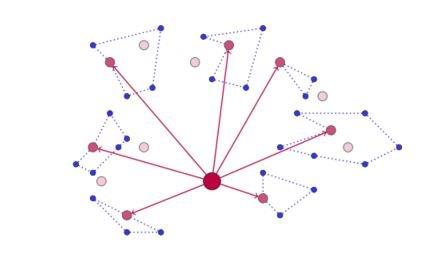
\includegraphics[width=.7\textwidth]{Fig1.jpg}
\caption{"Direct+Loop" Model}\label{fig:Model1}
\end{figure}
\newpage
 Fig.\eqref{fig:Model1} is the most common one in the LIRP. The model consist of set of suppliers (in this case there is only 1 plant), set candidate of depots (which depot should be opened and its location) and set of customers/retailers. The goods will be delivered to each plant directly to distribution centre and each distribution centre will do the routing through a number of customers. In the policy that we have to make is dealing based on the mentioned above: 
\begin{enumerate}
	\item Location : Where depots are should be opened including the cost to establish and operate. 
	\item Inventory : It is related to holding cost of each depot and how many quantity can be stored for each one of them. 
	\item Routing : Costs that are associated with delivering the goods from depots to retailers. 
\end{enumerate}
\begin{figure}
	\centering
	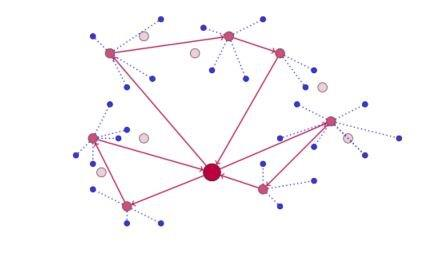
\includegraphics[width=.7\textwidth]{Fig2.jpg}
	\caption{"Loop+Direct" Model}\label{fig:Model2}
\end{figure}
\newpage
In this Fig.\eqref{fig:Model2},customers come directly to the depots and each customers are going to collect the demands through a set of candidate depots. In this case, a number of vehicles will do a routing through candidate depots based on the the customer demands that can be satisfied and then they are going back again to supplier to retrieve the demands. The policy that we have to make is dealing based on the mentioned above: 
\begin{enumerate}
	\item Location : Where depots are should be opened including the cost to establish and operate.
	\item Inventory : It is related to holding cost of each depot and how many quantity can be stored for each one of them.
	\item Routing : Costs that are associated with retrieving and distributing the goods to the customers. 
\end{enumerate}
This scenario works best in so many features, including:
	\begin{itemize}
		\item many independent customers 
		\item small frequent shipments
		\item possible consolidation at intermediate facilities
		\item agile networks, intermittent customers
	\end{itemize}	
To our best knowledges, there is not much study about this scenario, yet there is so many potential applications, including:
\begin{itemize}
	\item collection of breast milk
	\item reverse logistics, recovery of e-commerce goods
	\item distribution of dairy products
\end{itemize}

\section{Formulation of the "Direct+Loop" Model}

\subsubsection{Notations}\label{notations}
\begin{tabular}{ll}
\hline
Set & Definition \\
\hline
$I$ & Set of customers\\ 
$J$ & Set of distribution centers $j\in J$\\
$P$ & Set of plants (1 plant here)\\
$T=\left \{0,...,|T|\right \}$ & Set of time periods (days)\\
$V$ & Set of all nodes $V=P\cup I \cup J$\\
$V^*$ & Set of depots and clients $V^*=I \cup J$\\
$R$ & Set of routes\\
\hline
\end{tabular}
\newpage
\begin{tabular}{ll}
\hline
Data & Definition \\
\hline
$f_j$ & Fixed cost of opening distribution center $j\in J$\\ 
$Q$ & Capacity of vehicles (homogeneus fleet)\\ 
$d^t_i$ & Demand of customer $i /in I$ in period $t \in \left \{1,...,|T| \right \}$\\
$h^t_i$ & Holding cost at facility $i /in V^*$ in time period $t\in T$\\
$I_{i0}$ & Initial Inventory $i \in V^*$\\
$c_j$ & Cost of delivering distribution center $j\in J$ \\
$c_r$ & Cost of route $r\in R$\\
$\alpha_{ir}$ & 1 if route $r \in R$ visits facility $i\in V^*$. 0 otherwise\\
$I^{max}_j$ & Max inventory at distribution center $j \in J$\\
$I^{max}_i$ & Max inventory at client $i \in I$\\
\hline
\end{tabular}
\subsubsection{Variables}~\\
\begin{tabular}{ll}
\hline
\multicolumn{2}{l}{\textit{Binary Variables}}\\
$y_j$ & $\rightarrow$ 1 if distribution center $j$ is selected. 0 otherwise \\
$z^t_r$ & $\rightarrow$ 1 if route $r \in R$ is selected in period $t\in T$. 0 otherwise\\
$x^t_j$ & $\rightarrow$ 1 if distribution center $j\in J$ is delivered in time period $t$. 0 otherwise\\
\hline
\multicolumn{2}{l}{\textit{Continuous variables}}\\
\hline
$q^t_j$ & $\rightarrow$ quantity delivered to distribution center $j\in J$ in time period $t\in T$\\
$u^t_{ir}$ & $\rightarrow$ quantity delivered by route $r\in R$ to client $i \in I$ in time period $t \in T$\\
$I^t_i$ & $\rightarrow$ Inventory at facility $i\cup I\cup J$ in time period $t \in T$\\
\end{tabular}
\subsubsection{Assumptions}
In this model,we are dealing with:
\begin{itemize}
	\item Single Product
	\item Multi period
	\item Homogeneus Fleet
	\item The location of supplier and retailer are known, and ecah retailer has deterministic demand
	\item There are a set of potential sites for locating DCs, each has a capacity and fixed cost for opening a DC. 
\end{itemize}
\subsubsection{MIP defintion}
\begin{equation}
\text{min} \sum_{j\in J} f_j y_j 	+\sum_{t\in T} 
\left( \sum_{j\in J} c_j x^t_j + \sum_{r\in R} c_r z^t_r  + \sum_{t\in T} \sum_{i\in I} h^t_i I_i^t + \sum_{j\in J} h^t_j I_j^t \right) \label{objfunct}\
\end{equation}

\begin{align}
\text{s.t.}  &&\sum_{r\in R} \alpha_{ir} z^t_r 	&\leq 1 					&\forall i\in I, \forall t\in T  \label{const:customersingleroute}\\
		&&q^t_j 								&\leq Q x^t_j				&\forall j\in J, \forall t\in T \label{const:plantcapacity}\\
		&&x^t_j 								&\leq y_j   				&\forall j\in J, \forall t\in T\label{const:nounselectedroutes}\\
		&&\sum_{i\in I} u^t_{ir}   				&\leq  Q z^t_r 				&\forall r\in R, t\in T\label{const:capacityonroute}\\
		&&\sum_{r\in R} z^t_r 					&\leq K 					&\forall t\in T\label{const:fleetsizelimitation}\\
		&&z^t_r 								&\leq \sum_{j\in J}\beta_{jr} y_j 				&\forall r\in R, \forall t\in T\label{const:routestartsfromDC}\\
		&&I^{t-1}_j + q^t_j   					&=I^t_j +\sum_{r\in R}\beta_{jr} \left(\sum_{i\in I}u^t_{ir}\right) 	&\forall j\in J, \forall t\in T \label{const:flowconversationatDC}\\
		&&I^t_i				&=I^{t-1}_i+ \sum_{r\in R} u^t_{ir}-d^t_i 	&\forall i\in I, \forall t\in T\label{const:flowconservationatcustomer}\\
		&&I^t_i 			&\leq \min(I^{max}_i, \sum_{t'>t}^{t'<T}d^{t'}_i) 		&\forall i\in I, \forall t\in T\label{const:maxinventorycust}\\
		&&I^t_j									&\leq I^{max}_j y_j  				&\forall j\in J,\forall t\in T\label{const:capconstraintatdepot}\\	
		&&u_{ir}^t 			&\leq Q \alpha_{ir}						& \forall i\in I, \forall r\in R,\forall t\in T	\label{const:upperbound-u}\\
		&&q^t_j 						&\geq 0 					& \forall j\in J,\forall t\in T	\\
		&&u^t_{ir}						&\geq 0 					&\forall i\in I, \forall r\in R,\forall t\in T	\\
        &&y_{j}									& \in \{0,1\}, 				&\forall j\in J\label{12}\\	
		&&z^t_r									&\in \{0,1\}, 				&\forall r\in R, \forall t\in T						\label{13}\\
		&&x^t_{ij}								&\in \{0,1\},				&\forall i \in I, \forall j\in J,\forall t\in T		\label{14} \\
		&&I_j^t 								& \geq 0					&\forall j \in J, \forall t\in T \\
		&&I_i^t 								& \geq 0					&\forall i \in J, \forall t\in T \\
\end{align}

The objective function \eqref{objfunct} is to minimize the total cost including : Location Cost, Inventory Cost and Routing Cost.
The constraint \eqref{const:customersingleroute} states that every supplier is visited by at most one route for every period. 
Constraint \eqref{const:plantcapacity} is the capacity constraints between the plant and distribution center.
Constraint \eqref{const:nounselectedroutes} is to ensure that no routes is available to non selected distribution center. 
Constraint \eqref{const:capacityonroute} is capacity constraint on route r.
Constraint \eqref{const:fleetsizelimitation} is fleet size limitation.
Constraint \eqref{const:routestartsfromDC} is to ensure there is a route starts from selected depot.
Constraint \eqref{const:flowconversationatDC} is the flow conversation from distribution center j.
Constraint \eqref{const:flowconservationatcustomer} is the flow conversation at customer i. 
Constraint \eqref{const:maxinventorycust} is the maximum inventory at customer.
Constraint \eqref{const:capconstraintatdepot} is the capacity constraint at depot.

\section{Formulation of the Loop+Direct" Model }


\subsubsection{Notations}\label{subsection:notations2}
\paragraph{Data, sets and parameters}~\\
The data set and parameters is exactly the same with the first model in addition of :
\\
\\
\begin{tabular}{ll}
\hline
Data & Definition \\
\hline
$R$ & Set of routes\\ 
$c_r$ & Cost of route $r\in R$\\ 
$c_{ij}'$ & Cost of delivering customer $i\in I$ from distribution center $j\in J$\\
$\alpha_{jr}$ & If route $r\in R$ visit distribution center $j\in J$. 0 otherwise\\
\hline
\multicolumn{2}{l}{\textit{Continuous variables}}\\
\hline
$y_j$ & $\rightarrow$ if distribution center $j\ in J$ is selected. 0 otherwise\\
$z^t_r$ & $\rightarrow$ if route $r\in R$ is selected in period t. 0 otherwise\\
$x^t_{ij}$ & $\rightarrow$ if customer i is delivered by DC j in time period t\\
\end{tabular}
\subsubsection{Assumptions}
Same with the first model,in this scenario we are dealing with:
\begin{itemize}
	\item Single Product
	\item Multi period
	\item Homogeneus Fleet
	\item The location of supplier and retailer are known, and ecah retailer has deterministic demand
	\item There are a set of potential sites for locating DCs, each has a capacity and fixed cost for opening a DC. 
\end{itemize}
\subsubsection{MIP defintion}
\begin{align}
\text{minimize} &\sum_{j\in J} f_j y_j  +\sum_{t\in T} \left( \sum_{j\in J} c_r z_r^t + \sum_{i\in I} \sum_{j\in J} c_{ij}' x^t_{ij}\right) +\sum_{t\in T}\sum_{i\in V^*} h^t_i I_i^t\label{objfunct2}
\end{align}
\begin{align}
\text{s.t.} &&\beta_{jr} z^t_r 	&\leq y_j 									&\forall j&\in J, \forall r\in R, \forall t\in T\label{routeonselecteddepot}\\
		&&\beta_{jr}q^j_{rt} 	&\leq V z^t_r 										&\forall j&\in J, \forall r\in R, \forall t\in T\label{novehicleifrouteisnotopened}\\
		&&q^t_j 						&\leq M z^t_r 								&\forall j&\in J, \forall r\in R, \forall t\in T\label{capacityonroute}\\
		&&z^t_r 						&\leq K 									&\forall r&\in R,\forall t\in T\label{fleetsize}\\
		&&v^t_{ij}						&\leq Q x^t_{ij}								&\forall i&\in I, \forall j\in J, \forall t\in T\label{demandsatcustomer}\\
		&&v^t_{ij} 					&\leq \sum_{t'\geq t}^{t'\leq T} d^{t'}_i x^t_{ij}				&\forall i&\in I,\forall j\in J,\forall t\in T\label{demandsatcustomer1}\\
		&&x^t_{ij} 					&\leq y_j 									&\forall i&\in I, \forall j\in J, \forall t\in T\label{customerservedfromdepot}\\
		&&I^t_j 						&=I^{t-1}_j-q^t_j+\sum_{i\in I}v^t_{ij}\qquad 		&\forall i&\in I, \forall j\in J, \forall t\in T\label{flowconversationatdepot}\\
		&&I^t_i 						&=I^{t-1}_i+ \sum_{j\in J} v^t_{ij} - d^t_i 			&\forall i&\in I, \forall j\in J, \forall t\in T\label{flowconversationatcustomer}\\
		&&I^t_i 						&\leq\sum_{t'>t}^{t'\leq T} d^t_i 						&\forall i&\in I, \forall t\in T\label{maxinventory}\\
        &&I^t_i						&\leq I_i									&\forall i&\in I, \forall t\in T\label{capacityatcustomers}\\
       	&&I^t_j						&\leq I_j y_j									&\forall j&\in J, \forall t\in T\label{capacityatdepot}\\
        &&y_j						&\in\{0,1\}, 								&\forall j &\in J\label{boolean var1}\\
   		&&z^t_r 						&\in \{0,1\},	 							&\forall r &\in R, \forall t\in T\label{boolean var2}\\
		&&x^t_{ij} 					&\in \{0,1\}, 								&\forall i &\in I, \forall j\in J,\forall t\in T\label{boolean var3}\\
		&&I^t_i, I^t_j					&\geq 0 									&\forall i&\in I, \forall j\in J,\forall t\in T\label{const1}\\	
		&&q^t_i, I^t_j					&\geq 0 									&\forall i&\in I, \forall j\in J,\forall t\in T\label{const2}				
\end{align}
The objective function \eqref{objfunct2} is to minimize the total cost including : Location Cost, Inventory Cost and Routing Cost.
Constraint \eqref{routeonselecteddepot} state that every distribution center can be visited at most one route for every period. 
Constraint \eqref{novehicleifrouteisnotopened} is there is no vehicle at routes if they are not selected to make delivery to customers. 
Constraint \eqref{capacityonroute} is the capacity constraint on selected routes. 
Constraint \eqref{fleetsize} is the fleet size limitation.
Constraint \eqref{demandsatcustomer} and \eqref{demandsatcustomer1} are capacity of demands at customer if they are being delivered at route $r$ in period $t$.
Constraint \eqref{customerservedfromdepot} is a customer is served from a selected distribution center.
Constraint \eqref{flowconversationatdepot} is the flow conversation at distribution center $j$.
Constraint \eqref{flowconversationatcustomer} is the flow conversation at customer $i$.
Constraint \eqref{maxinventory} is maximum inventory at customers.
Constraint \eqref{capacityatcustomers} is maximum capacity for each customer.
Constraint \eqref{capacityatdepot}is maximum capacity for each depot and to assure that there is no inventory at non selected depot.


\section{Numerical results}
The algorithm is coded in Java and the MIP model is solved with CPLEX. We generated small instances first with 5 customers up until 15 customers with 3 depots and 5 periods. 
\begin{table}[ht]
	\begin{tabular}{{ |p{2cm}||p{2cm}|p{2cm}|p{2cm}||p{2cm}||p{2cm}|  }}  
		\hline
		Size of Instances & Fixed Cost & Ordering Cost & Routing Cost & Inventory Cost & Optimal Value\\ 
		\hline
		5 & cell2 & cell3 & cell4 & cell  & cell6 \\ 
		10 & cell2 & cell3 & cell4 & cell & cell6 \\
		15 & cell2 & cell3 & cell4 & cell & cell6 \\ 
		\hline
	\end{tabular}
		\caption{Results ILRP Model 1}
		\label{table:2}
\end{table}

\begin{table}[ht]
		\begin{tabular}{{ |p{2cm}||p{2cm}|p{2cm}|p{2cm}||p{2cm}||p{2cm}|  }} 
		\hline
		Size of Instances & Fixed Cost & Ordering Cost & Routing Cost & Inventory Cost & Optimal Value\\ 
		\hline
		5 & cell2 & cell3 & cell4 & cell  & cell6 \\ 
		10 & cell2 & cell3 & cell4 & cell & cell6 \\
		15 & cell2 & cell3 & cell4 & cell & cell6 \\ 
		\hline
	\end{tabular}
	\caption{Results ILRP Model 2}
	\label{table:3}
\end{table}
\section{Conclusion and further research}
We analyze between the two model, the first one which is the most common one in ILRP and the second one which we are proposing and compare them based on number of instances. Our results show that bla bla bla. For the further research :we can try to solve it with a heuristic method for larger instances.

    
\section{Bibliography}
\printbibliography

\end{document}